\graphicspath{{../04ClassicalPhysics/pics/}}

\chapter{Classical Physics}\label{ch:ClassicalPhysics}
\lettrine[lines=2]{\color{darkocre}T}{he} concept of
\emph{operators}\index{Operator} extends the idea of functions. An unary numeric
function $f$ takes some numeric value $x$ as an input  and produces
another numeric value $y$:
\[
f\,x=y\quad \textrm{ or } \quad x\overset{f}{\longrightarrow} y\,.
\]
In mathematical jargon, $f$ \emph{maps} $x$ into $y$.

Similarly, we can study
 functions that \emph{operate} on arrows/vectors, yielding other
 arrows/vectors. The
parallel between unary functions over numbers and unary operators over
vectors is highlighted in the Figure \ref{fig:arrowsOperatorGeneral}.

\begin{figure}[htbp]
  \centering
  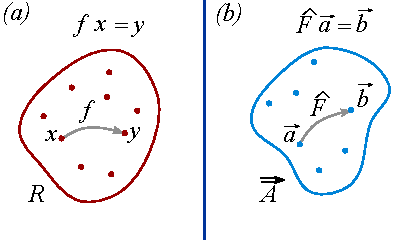
\includegraphics[scale=1.0]{arrowsOperatorGeneral}
  \caption{Operators extend the idea of functions. (a) An unary
    function $f$ can be applied to a number $x$ to produce
    another number $y$. (b) An unary operator $\op{F}$ can be applied to a vector
    $\vec{a}$ to yield another vector $\vec{b}$.}
  \label{fig:arrowsOperatorGeneral}
\end{figure}

\section{Operators on Arrows}\label{sec:OperatorsOnArrow}
An action of an operator $F$ on arrows can be represented symbolically
as an equation:
\[
F\,\vec{a}=\vec{b}\:.
\]
Often a ``hat'' is placed on top of an operator\footnote{In Quantum
Mechanics, for example.}, to emphasize that it is different from
numeric function:
\[
\colorboxed{red}{
  \op{F}\,\vec{a}=\vec{b}\:.
}
\]

%\begin{tcolorbox}[colback=white!85!ocre, title=Simple Operators]
\begin{bio}\faBook\,\,\bem{Simple Operators}\\
It is easy to come up with examples of operators:

\begin{itemize}
\item\phantom{x}

\item Unit operator (or \emph{identity} operator), such that
  \[
  \op{I}\,\vec{a}=\vec{a}\,.
  \]

\item ``Zeroing'' operator that maps every vector into a zero
  vector:
  \[
  \op{0}\, \vec{a} = \vec{0}\,.
  \]

\item Scaling operator, such that
  \[
  \op{S}_5\,\vec{a} = 5\vec{a}\,.
  \]

\item Rotation operator, such that
  \[
  \op{L}\,\vec{a} = \vec{b}\,,
  \]
  where $\vec{b}$ is rotated by $45^\circ$ counter-clockwise relative to the
  vector $\vec{a}$.

\end{itemize}
\end{bio}
%\end{tcolorbox}


To fully describe an operator, we must describe how it acts \emph{on
every} arrow. In general, this
requires an \emph{infinite} amount of information, since there are
infinite number of arrows and the action of $F$ on different arrows
might be different\footnote{Simple operators given before are special
cases when it is easy to describe action of operators on \emph{all}
vectors.}. Describing the action of a general operator in
graphical terms using arrows is a hopeless task. This is the case
where component\index{Operator!components}
representation of arrows saves the day.

If we fix a basis $\lbrace \vec{e}_i\rbrace$, then every vector gets
an algebraic representation as a set of components:
\[
\vec{a}\qquad\overset{\lbrace \vec{e}_k\rbrace}{\longrightarrow}\qquad a_i\,,
\]
\[
\vec{b}\qquad\overset{\lbrace \vec{e}_k\rbrace}{\longrightarrow}\qquad b_j\,.
\]
Now to describe the action of an operator $\op{F}$ on the vector
$\vec{a}$ we can specify the components of the result $b_j$ for
arbitrary components of the input $a_i$. For vectors in a plane, we have
\[
b_1 = F_{1}\,a_{1}\, a_2
\]
and
\[
b_2 = F_{2}\,a_1\,a_{2}\,.
\]
Thus, a pair of binary numeric functions $F_{1}$ and $F_{2}$ is
sufficient to describe an operator. A situation significantly
simplifies in the case of very important \emph{linear operators} which
we will discuss soon in Section \label{sec:LinearOperators}.

\begin{flushleft}
  {\bf Examples}
\end{flushleft}
Let us take a closer look at a couple of operators. While studying
these examples we must keep in mind that the relations between
components are \emph{specific to basis} and will change if we change the
basis. The question of how exactly the relation between components
changes will be addressed later in Section
\ref{sec:ComponentTransformation} for the simplest types of operators.

The first operator acts on the components as follows:
\[
b_1 = a_1 + a_2\,,
\]
\[
b_2 = a_1 * a_2\,.
\]
To illustrate these relations visually, we can start with arrows of
equal lengths but pointing in all directions. The tips of such arrows
will lie on a circle, as shown in the Figure \ref{fig:operatorActionV1}
using blue dotted lines. The tips of all output arrows
$\vec{b}=\op{F}\,\vec{a}$ lie on a curve shown in
the Figure \ref{fig:operatorActionV1} using solid red line.
\begin{figure}[htbp]
  \centering
  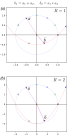
\includegraphics[scale=1.0]{operatorAction_v1}
  \caption{The action of the operator $\op{F}$ on planar arrow-vectors
    $\vec{a}$. To demonstrate how $\op{F}$ acts on arrows of different
  directions and lengths, we consider what happens to the circles of
  two different radii.}
  \label{fig:operatorActionV1}
\end{figure}
In the first example the arrows tracing the circle of the radius
$R=1$ are transformed into arrows tracing a curve that looks like
parabola.
%\begin{tcolorbox}[colback=white!85!ocre, title=Problem]
\begin{exercise}\label{exe:CircleToParabola}
Show that when the components of the output arrow $\vec{b}$ are given
by
\[
b_1 = a_1 + a_2\,,
\]
\[
b_2 = a_1 * a_2\,,
\]
then the circe with the radius $R$ becomes a parabola described by the
equation
\[
b_2 = b^2_1/2 - R^2/2\,.
\]
\end{exercise}
%\end{tcolorbox}

In the second example the operator $\op{G}$ acts on the components as follows:
\[
b_1 = a_1 - a_2\,,
\]
\[
b_2 = -a^2_1 * a_2\,.
\]
\begin{figure}[htbp]
  \centering
  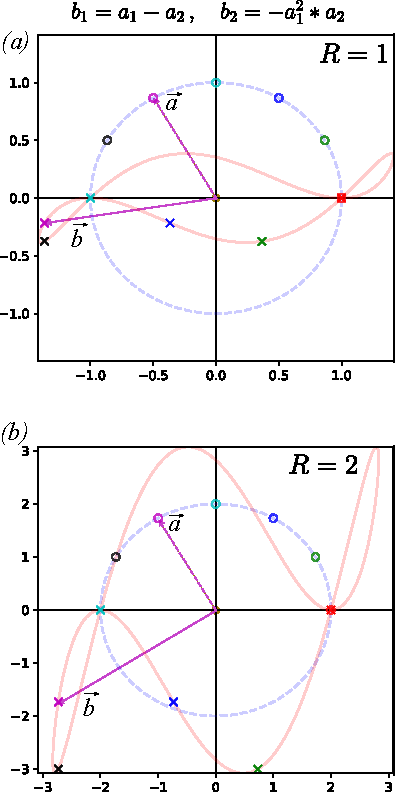
\includegraphics[scale=1.0]{operatorAction_v2}
  \caption{An action of an operator $\op{G}$ on a planar vector
    $\vec{a}$. To demonstrate how $\op{G}$ acts on arrows of different
  directions and lengths, we consider what happens to the circles of
  two different radii.}
  \label{fig:operatorActionV2}
\end{figure}
The effect of this operator on the arrows forming a circle is
illustrated in the Figure \ref{fig:operatorActionV2}. It seems that
increasing the radius of the circles does not substantially change its
``image'' (solid red line)  and only ``stretches'' the output curve
both horizontally and vertically.
%\begin{tcolorbox}[colback=white!85!ocre, title=Problem]
%% \begin{exercise}\label{exe:scalingTransformation}
%% Show that if the components of the output arrow $\vec{b}$ are given
%% by
%% \[
%% b_1 = a_1 - a_2\,,
%% \]
%% \[
%% b_2 = -a^2_1 * |a_2|\,.
%% \]
%% then when the scale of both $a_1$ and $a_2$ increases by a factor of 2
%% the value of the component $b_1$ also increases by 2, while the
%% component $b_2$ increases 8 times.

%% \emph{Hint}: Write the components of the input arrows that form a
%% circles as
%% \[
%% a_1 = R \cos\theta\,,\qquad a_2 = R\sin\theta\,.
%% \]
%% \end{exercise}
%% %\end{tcolorbox}
\begin{mybio}{Nonlinear and Linear Operators}
  The operators $\op{F}$ and $\op{G}$ are examples of rather
  complicated operators. They are
  \emph{nonlinear}\index{Operator!nonlinear} because they lack
  the simple property of \emph{linearity} (we will learn about it
  soon in Section \ref{sec:LinearOperators}.)

  Linear operators\index{Operator!linear} connect components of input
  and output vectors in a simple way:
  \[
   b_1 = A\,a_1 + B\, a_2\,,\quad b_2 = C\,a_1 + D\, a_2\,.
   \]
   Here $A,\, B\,, C\,, D$ are numbers. Different linear operators
   differ only in the values of these numbers. Despite their
   simplicity, linear operators are powerful and widely used.
\end{mybio}

\begin{figure}[htbp]
  \centering
  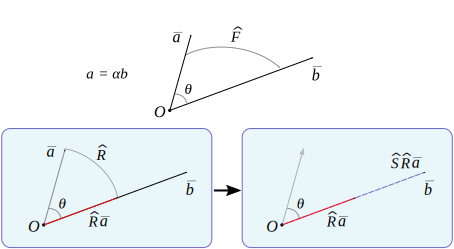
\includegraphics[scale=1.0]{operatorsAction}
  \caption{An action of an operator $\op{F}$ on a planar vector
    $\vec{a}$ can be described by the sequence of rotation $\op{R}$
    and scaling $\op{S}$: $\op{F}=\op{S}\circ\op{R}$.}
  \label{fig:operatorsAction}
\end{figure}
Since two arrows can differ only in their magnitude (length) and
directions, the action of an operator
 can be represented by a combination of two steps: rotation and
 scaling; see the Figure \ref{fig:operatorsAction}. The order of scaling
 and rotation does not matter:
 \[
 \op{F}=\op{S}\circ\op{R} = \op{R}\circ\op{S}\,.
 \]
 As our next step, we will study rotation operators in more details.

\subsection{Rotation Operator}
A simple non-trivial\footnote{An example of a trivial operator is the identity
operator $\op{I}$ which does not change the input vector: $\op{I}
\vec{a} = \vec{a}$. Another example is the operator that always
returns ``zero''-arrow: $\op{0}\,\vec{a}=\vec{0}$.} operator rotates
a vector by some angle, as demonstrated in the Figure \ref{fig:operatorsRotator}.
\begin{figure}[htbp]
  \centering
  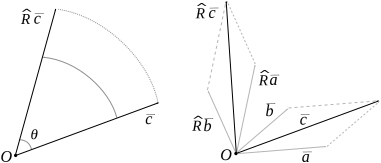
\includegraphics[scale=1.0]{operatorsRotator}
  \caption{The action of the rotation operator $\op{R}$ on a planar vector
    $\vec{a}$ results in the rotation by a specified angle
    $\theta$. Such rotation posseses an important property: $\op{R}\,(\vec{a}+\vec{b})=\op{R}\,\vec{a}+\op{R}\,\vec{b}$.}
  \label{fig:operatorsRotator}
\end{figure}
Strictly speaking, there are infinite number of such operators, one
for each rotational angle $\theta$.

An important property of any rotation
operator\index{Operator!rotation} is that it preserves
some relations between arrows. For example, given a vector
\[
\vec{c} = \vec{a} + \vec{b},
\]
its ``image'' $(\op{R}\,\vec{c})$ can be constructed from rotated
vectors $(\op{R}\,\vec{a})$ and $(\op{R}\,\vec{b})$:
\[
\op{R}\,\vec{c} =\op{R}\,(\vec{a} + \vec{b}) = (\op{R}\,\vec{a}) + (\op{R}\,\vec{b}).
\]
This property is the consequence of two features of the rotation
operator: 1) it does not change the length of a vector; 2) it rotates
every vector by the same amount, thus keeping the relative angle between any
two vectors intact, as shown in the see Figure \ref{fig:operatorsRotator}.

Another important property of rotation operators is an obvious one:
\[
\op{R}\, (\alpha \vec{a}) = \alpha (\op{R}\,\vec{a})\,.
\]
Rotation operators represent a subset of a larger set of important
operators -- \emph{linear operators}.

\section{Linear Operators}\label{sec:LinearOperators}

\emph{Linear operators}\index{Operator!linear} are operators with a
simple but important
property of \emph{linearity}\index{Linearity}. Two things are required
for a linear operator $\op{L}$:
\[
\colorboxed{red}{
  \op{L}\,(\vec{a}+\vec{b})=(\op{L}\,\vec{a})+(\op{L}\,\vec{b})
  }
\]
and
\[
\colorboxed{red}{
  \op{L}\,(\alpha\vec{a})=\alpha(\op{L}\,\vec{a})\,.
}
\]
Rotation operators satisfy these requirements, as we established in
the previous section.

To represent linear operators numerically using basis arrows requires
very little information. Indeed, for a general arrow
$\vec{a}=a_1\vec{e}_1+a_2\vec{e}_2$ the action of the operator
$\op{L}$ can be written as
\[
\op{L}\,(a_{1}\vec{e}_{1}+a_{2}\vec{e}_{2})=\lbrack
\op{L}\,(a_{1}\vec{e}_{1})\rbrack+\lbrack
\op{L}\,(a_{2}\vec{e}_{2})\rbrack=a_{1}(\op{L}\,\vec{e}_{1})+a_{2}(\op{L}\,\vec{e}_{2})\,.
\]
Thus, to define the action of the linear operator $\op{L}$ on an
arbitrary arrow $\vec{a}$, it is sufficient to define its action on the
basis arrows $\vec{e}_1$ and $\vec{e}_2$.

Operator $\op{L}$ acts on arrows to yield other arrows. Thus, we can
write
\[
\op{L}\,\vec{e}_{1} = \vec{f}_{1}\, \textrm{ and } \op{L}\,\vec{e}_{2} = \vec{f}_{2}\,.
\]
Like any other vectors, the vectors $\vec{f}_{1}$ and $\vec{f}_{2}$
can be written in terms of the basis vectors:
\[
\vec{f}_{1}=l_{1}\vec{e}_{1}+l_{2}\vec{e}_{2}\,,
\]
\[
\vec{f}_{2}=l_{3}\vec{e}_{1}+l_{4}\vec{e}_{2}\,.
\]
These equations can be written more compactly if we improve the notation.
Firstly, instead of numbers $l_{1}\,,l_{2}\,,l_{3}\,,l_{4}$ we will
write
\[
\op{L}\,\vec{e}_{1}=L_{11}\vec{e}_{1}+L_{12}\vec{e}_{2}
\]
and
\[
\op{L}\,\vec{e}_{2}=L_{21}\vec{e}_{1}+L_{22}\vec{e}_{2}\,.
\]
Notice how the subscript indices match nicely with the indices of
the basis arrows: The first subscript index of $L_{ij}$ corresponds to
the basis vector being acted on, while the second index corresponds to
the basis vectors being multiplied by $L_{ij}$. The second step is to
use the summation agreement:
\[
\op{L}\,\vec{e}_{1}=L_{1j}\vec{e}_{j},
\]
\[
\op{L}\,\vec{e}_{2}=L_{2j}\vec{e}_{j}.
\]
Finally, we can write the most compact form:
\begin{equation}
  \colorboxed{red}{
    \op{L}\,\vec{e}_{i}=L_{ij}\vec{e}_{j}.
    }
\end{equation}
In summary, the action of a linear operator $\op{L}$ on the basis arrows
(and, consequently, on \emph{any} arrow) is completely determined by its
components $L_{ij}$-- just four numbers for arrows in a
plane\footnote{In a space of $N$ dimensions the number of components
is, in general, equal to $N^2$.}.

The components\index{Operator!components} of a linear operator $\op{L}$ are
specific to the basis.
This is completely analogous to the components of arrow-vectors. Indeed,
the use of a basis translates arrows and linear operators from the
graphical world of drawings into the algebraic world of numbers:
\[
\vec{a}\overset{\{\vec{e}_{1}\,,\vec{e}_{2}\}}{\longrightarrow}a_{i}\,,
\]
\[
\op{L}\,\overset{\{\vec{e}_{1}\,,\vec{e}_{2}\}}{\longrightarrow}L_{ij}\,.
\]

%\begin{tcolorbox}[colback=white!85!ocre, title=Simple Linear Operators]
\begin{mybio}{Simple Linear Operators}
Four simple types of linear operators can be defined without specifying their
components:
\begin{itemize}
  \item\phantom{x}
\item Unit operator, such that $\op{I}\,\vec{a}=\vec{a}$.
\item ``Zeroing'' operator that maps every vector into a zero
  vector:
  \[
  \op{0}\, \vec{a} = \vec{0}\,.
  \]
\item Scaling operators, such that $\op{S}\,\vec{a} = \alpha\vec{a}$
  for some specified value $\alpha$.
\item Rotation operators, such that $\op{R}_\theta\,\vec{a} = \vec{b}$, where
  $\vec{b}$ is simply rotated by specified angle $\theta$.
\end{itemize}
To find the components of any operator we must see how it acts on
basis vectors. Let's see how this works for the scaling operator
$\op{S}$ described above:
\[
\op{S}\,\vec{e}_1 = \alpha\vec{e}_1 + 0\vec{e}_2\,,
\]
\[
\op{S}\,\vec{e}_2 = 0\vec{e}_1 + \alpha\vec{e}_2\,.
\]
From these equations we can read the components $S_{ij}$ and write
them in matrix form:
\[
\op{S} =
\begin{pmatrix}
  S_{11} & S_{12}\\
  S_{21} & S_{22}
\end{pmatrix} =
\begin{pmatrix}
  \alpha & 0\\
  0 & \alpha
\end{pmatrix}\,.
\]
Similar approach can be used to find the components of any linear operator.
\end{mybio}
%\end{tcolorbox}

%\begin{tcolorbox}[colback=white!85!ocre, title=Problem]
\begin{exercise}\label{exe:normalizationOperator}
Consider an operator $\op{N}$ which ``normalizes'' an arrow -- returns
an arrow of unit length pointing in the same direction as the
original one. For example:
\[
\op{N}\,\vec{a} = \vec{u}_a = \frac{\vec{a}}{a}\,.
\]
Is it a linear operator?
\end{exercise}
%\end{tcolorbox}
\begin{mybio}{$\op{J}$-operator}
Operator that rotates any vector by $90$ degrees has a special
notation (it will be heavily used in Sections \ref{sec:CompoundNumbers}
and \ref{sec:HamiltonianMechanics}):
\[
\op{R}_{\pi/2} = \op{J}\,.
\]

It is instructive to see how this operator acts on orthonormal basis
$\lbrace \vec{e}_i\rbrace$:
\[
\op{J}\,\vec{e}_1 = \vec{e}_2 = 0\,\vec{e}_1 + 1\,\vec{e}_2
\]
and
\[
\op{J}\,\vec{e}_2 = -\vec{e}_1 = -1\,\vec{e}_1 + 0\,\vec{e}_2\,.
\]
From the last two expressions we can find the components of the
$\op{J}$-operator:
\[
J_{ij}=
\begin{pmatrix}
  J_{11} & J_{12}\\
  J_{21} & J_{22}
\end{pmatrix} =
\begin{pmatrix}
  0 & 1\\
  -1 & 0
\end{pmatrix}\,.
\]
Here we used \emph{matrix}\index{Matrix} form of presenting the
components of linear operators. In this form, the first index of the
components corresponds to the row in the matrix-table, and the second
index corresponds to the column.

Another important property of this operator can be seen when we act on
any vector twice:
\[
\op{J}\,(\op{J}\,\vec{a}) = -\vec{a}\,.
\]
Indeed, rotating any vector twice by 90 degrees results in total
rotation by 180 degrees -- the direction of the original vector is
flipped. What we showed is that the sequence $\op{J}\circ\op{J}$ is
the same as the operator $(-\op{I})$:
\[
\colorboxed{red}{
  \op{J}\circ\op{J} = -\op{I}\,.
}
\]
\end{mybio}


\section{Plotting Linear Operators}
A numeric unary function
\[
f\, x = y
\]
can be represented graphically as
a plot ``$y\,vs\, x$''. In this plot we indicate a value $y$
\emph{for each value of} $x$.

Linear operators of the type
\[
\op{L}\,\vec{a} = \vec{b}
\]
also allow graphical representation\index{Operator!plotting}. We can,
for example, draw an
arrow $\vec{b}$ \emph{for each value of} $\vec{a}$. The input vector
$\vec{a}$ can vary both its lengths and direction. For a linear
operator $\op{L}$ the change in length of the input vector $\vec{a}$
is handled trivially:
\[
\op{L}\,(\alpha \vec{a}) = \alpha (\op{L}\,\vec{a})\,.
\]
In words: To find the action of a linear operator on a scaled vector
we first apply the operator to the original vector and then scale the
result. It also follows that all vectors $\op{L}\,(\alpha \vec{a})$
corresponding to different values of the scale factor $\alpha$ are
\emph{parallel} -- they are all parallel to the vector
$\vec{b}=\op{L}\,\vec{a}$.

The preceding considerations show that to describe the action of a
linear operator on
various input vectors we can focus only on vectors with unit lengths,
but pointing in all possible directions. The tips of all such vectors
form a unit circle, as illustrated in the Figure
\ref{fig:linearOperatorAction}.
\begin{figure}[htbp]
  \centering
  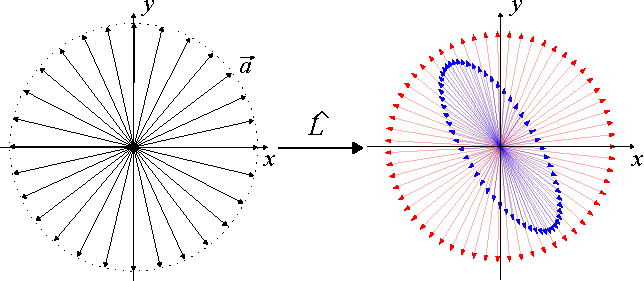
\includegraphics[scale=1.0]{linearOperatorAction}
  \caption{Input vectors for a linear operator can vary in
    direction. In this example the components of the operator are:
    $L_{11}=2/10\,, L_{12}=3/10\,, L_{21}=5/10\,,L_{22}=-7/10\,.$}
  \label{fig:linearOperatorAction}
\end{figure}

For linear operators it is sufficient to plot only the half of the circle,
since
\[
\op{L}\,(-\vec{a}) = -(\op{L}\,\vec{a})\,.
\]
In other words, the missing half is the inverted copy of the original half.
An illustration of this is given in the Figure \ref{fig:linearOperatorActionHalf}

\begin{figure}[htbp]
  \centering
  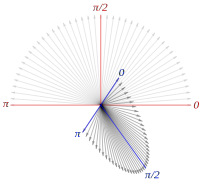
\includegraphics[scale=1.0]{linearOperatorActionHalf}
  \caption{To graphically describe a linear operator we can specify
    how it acts on vectors from the top half of the circle (the bottom
    is found by inverting the top). In this
    example the components of the operator are:
    $L_{11}=2/10\,, L_{12}=3/10\,, L_{21}=5/10\,,L_{22}=-7/10\,.$}
  \label{fig:linearOperatorActionHalf}
\end{figure}
\begin{figure}[htbp]
  \centering
  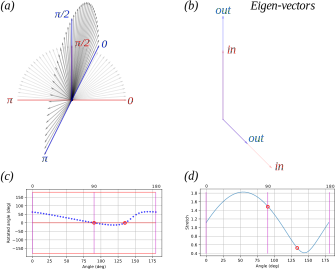
\includegraphics[scale=1.0]{linearOperatorActionZ}
  \caption{Graphical representation of a linear operator $\op{L}$ with components:
    $L_{11}=5/10\,, L_{12}=2\,, L_{21}=0\,,L_{22}=3/2\,.$ (a) The
    effect of the operator on unit-length arrows with direction from
    $0^\circ$ to $180^\circ$; (b) Two special arrow-vectors that do
    not change their direction under the action of the operator
    $\op{L}$. The operator simply scales the arrows. Such vectors
    are called \emph{eigen-vectors}\index{Vector!eigen} of the operator;
    (c) Horizontal axis: initial orientation of the unit-length arrow;
    vertical axis: rotation angle of each unit-length arrow. Two
    special angles are highlighted. For each special angle the arrow is not
    rotated. Such arrows are called eigen-vectors of the operator $\op{L}$;
    (d) Horizontal axis: initial orientation of the unit-length arrow;
    vertical axis: the scaling factor of each unit-length arrow.}
  \label{fig:linearOperatorActionZ}
\end{figure}

Another linear operator, with components
$L_{11}=5/10\,,L_{12}=2\,,L_{21}=0\,,L_{22}=3/2$, is graphically
represented in the Figure \ref{fig:linearOperatorActionZ}. In the
Figure \ref{fig:linearOperatorActionZ}(a) the action of the operator
on unit vectors from the top half-plane is shown, with the missing part
(bottom half-plane) is easily constructed by inverting the transformed
part through the origin. Although not easily seen, there are two
pairs of vectors\footnote{Two vectors and their reversed images.} that
are transformed rather simply by this linear
operator -- they are scaled without rotation. Two such vectors
are shown in the Figure \ref{fig:linearOperatorActionZ}(b). Such vectors are
called \emph{eigen-vectors}\index{Vector!eigen} of a given
operator. Eigen-vectors are
discussed in more details in the next section.

Another way to graphically represent a linear operator is to plot two
functions: 1) How much an input unit vectors gets rotated; 2) How much
an input unit vector gets stretched. This is done in the Figure
\ref{fig:linearOperatorActionZ}(c) and (d). From the Figure
\ref{fig:linearOperatorActionZ}(c) it can be seen that there are two
unit vectors that are not rotated by the operator (rotation angle is
zero for the input vectors at 90 degrees and at about 130 degrees or
310=130+180 degrees).

Eigen-vectors are important and finding them for a given linear
operator is an often encountered problem. It is called
\emph{eigen-vector problem} or \emph{eigen-problem} for short.


\section{Eigen-Problem*}
\emph{Eigen-vectors of a linear operator}\index{Vector!eigen} are
special vectors that are not
rotated by the operator, eigen-vectors can only be scaled. This requirement
can be expressed using a simple equation:
\[
\colorboxed{red}{
  \op{L}\,\vec{a} = \alpha\vec{a}\,,
}
\]
or, if there exists another eigen-vector $\vec{b}$ different from
$\vec{a}$:
\[
\op{L}\,\vec{b} = \beta\vec{b}\,.
\]
Here the numbers $\alpha$ and $\beta$ specify the scaling
coefficients. The
equations given above are called \emph{eigen-problem equations}. The
vectors $\vec{a}$ and $\vec{b}$ are called \emph{eigen-vector}, the
scaling factors $\alpha$ and $\beta$ are called
\emph{eigen-values}\index{Eigen-value}. In general, $\alpha\ne \beta$,
as illustrated in
the Figure \ref{fig:linearOperatorActionZ}(b).

%% A linear operator may have several eigen-vectors, and each
%% eigen-vector may
%% scale differently. To emphasize this point, eigen-vector is written
%% with the corresponding eigen-value as the subscript. Using this
%% notation, the eigen-problem equation can be written as follows:
%% \[
%% \op{L}\,\vec{a}_\alpha = \alpha\vec{a}_\alpha\,.
%% \]

Not all linear operators have eigen-vectors. A simple example is the
operator of rotation by a finite angle:
\[
\op{R}_\theta \,\vec{a} \ne \alpha \vec{a}\,.
\]
Simply speaking, it is impossible to rotate a vector without changing
its direction.

All ``well-behaved'' linear operators\footnote{We will encounter
ill-behaved linear operators in the next section.} (excluding rotation
operators like $\op{R}_\theta$) have the same number of  eigen-vectors
as the
number of basis vectors. Any ``well-behaved'' linear operator that
operates on vectors in a plane has two eigen-vectors, as illustrated
in the Figure \ref{fig:linearOperatorActionZ}(b). Operators acting on
vectors in three dimensions may have up to three eigen-vectors.

It is possible to find linear operators that have fewer eigen-vectors
than the number of basis vectors. Such operators are called
\emph{degenerate operators}. They are important and we will consider them
next for the special case of two dimensions.

\section{Degenerate Linear Operators}

In some special cases, a linear operator $\op{L}$, when applied to the
basis arrows $\vec{e}_{1}$ and $\vec{e}_{2}$ can produce parallel
arrows:
\[
(\op{L}\,\vec{e}_{1})\, \parallel \,(\op{L}\,\vec{e}_{2})
\]
or
\[
\op{L}\,\vec{e}_{1}=\lambda(\op{L}\,\vec{e}_{2})
\]
for some number $\lambda$.

Using components notation, this condition can be written as follows:
\[
L_{11}\vec{e}_{1}+L_{12}\vec{e}_{2}=\lambda L_{21}\vec{e}_{1}+\lambda L_{22}\vec{e}_{2}\,.
\]
The vector on the left-hand side is the same vector as on the right-hand
side if they have the same components in the given basis. Therefore,
we must equate corresponding components:
\[
L_{11}=\lambda L_{21}
\]
and
\[
L_{12}=\lambda L_{22}\,.
\]
Cross-multiplying these equations, we obtain
\[
\lambda L_{11}L_{22}=\lambda L_{12}L_{21}\,,
\]
from which follows
\[
L_{12}L_{21}-L_{11}L_{22}=0\,.
\]
Linear operator satisfying this condition is called
\emph{degenerate}\index{Operator!degenerate} for the reasons
explained below.

%\begin{tcolorbox}[colback=white!90!ocre, title=Problem]
\begin{exercise}\label{exe:degenerateCollapse}
Show that a degenerate linear operator $\op{L}$  ``collapses'' all
vectors onto the same line, i.e. all $(\op{L}\,\vec{a})$ have the same
direction.
\end{exercise}
%\end{tcolorbox}


Later in Section \ref{sec:Projectors} we will encounter a whole class
of useful degenerate linear
operators, called \emph{projectors}\index{Operator!projector}, whose
job is to project any
vector onto a specified direction.

\subsection{Determinant of a Linear Operator}

The quantity
\[
\colorboxed{red}{
  D=L_{12}L_{21}-L_{11}L_{22}
  }
\]
computed from the components of a linear operator is called its
\emph{determinant}\index{Determinant}. Determinant
 is one of important characteristics of a linear
operator, analogous to how the length of a vector is its important
characteristic.

Determinant has a clear geometric meaning which can be seen
from the action of the operator $\op{L}$ on orthonormal basis, as
illustrated in the Figure \ref{fig:operatorsDeterminant}.
\begin{figure}[htbp]
  \centering
  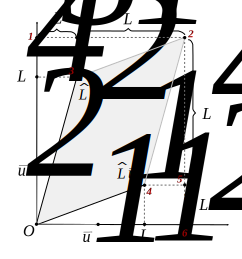
\includegraphics[scale=1.0]{operatorsDeterminant}
  \caption{A linear operator $\op{L}$ transforms basis vectors
    $\vec{u}_i$ into $\vec{v}_i=\op{L}\,\vec{u}_i$. For non-degenerate
  operator the vectors $\vec{v}_i$ form sides of a parallelogram with
  non-zero area $A=L_{12}L_{21}-L_{11}L_{22}$.}
  \label{fig:operatorsDeterminant}
\end{figure}
Denoting $L_{11} = L_{1}$, $L_{12} = L_2$, $L_{21} = L_3$, and
$L_{22} = L_4$, we can calculate the area of the parallelogram
built from the vectors $(\op{L}\,\vec{u}_1)$ and
$(\op{L}\,\vec{u}_2)$ as follows:
\[
A = (L_1 + L_3)(L_2 + L_4) - 2( L_1L_2/2 + L_3L_4/2 + L_2L_3)\,.
\]
It is simply the area of the rectangle $O126$ minus the areas of two
rectangles with sides $L_2$ and $L_3$, together with two pairs of
triangles.

After simplification the last equation reduces to
\[
A = L_1L_4-L_2L_3 = L_{11}L_{22} - L_{12}L_{21}.
\]

Thus, the determinant of a
linear operator $L$ equals to the ratio of the area of the parallelogram built
from the vectors $(\op{L}\,\vec{u}_1)$ and $(\op{L}\,\vec{u}_2)$ to the
 area of the parallelogram built from the unit vectors
$\vec{u}_1$ and $\vec{u}_2$. Obviously,
for a degenerate linear operator, this ratio is zero, since all arrows
``collapse'' onto a single direction.

%\begin{tcolorbox}[colback=white!90!ocre, title=Determinant]
\begin{mybio}{Determinant}
For arrow-vectors in three dimensions and higher, we also have linear
operators. The meaning of determinant in these higher-dimensional
cases remains similar: Determinant expresses the ratio of
\emph{volumes} built from basis vectors $\vec{e}_1\,
,\vec{e}_2\,\ldots\,,\vec{e}_n$, and from their ``transformed''
versions
$\op{L}\vec{e}_1\,,\op{L}\vec{e}_2\,\ldots\,,\op{L}\vec{e}_n$.
\end{mybio}
%\end{tcolorbox}


\section{Using Operator Components}
It is possible, and often convenient, to work with a linear operator
using only its components, without referring to arrows or some other
graphical representation.

The action of a linear operators $\op{L}$ on a vector $\vec{a}$ can be
written in terms of components\index{Operator!components}:
\[
\op{L}\,\vec{a} = \op{L}\,(a_i\vec{e}_i) =a_i\,(\op{L}\,\vec{e}_i) = a_i (L_{ij}\vec{e}_j).
\]
On the other hand
\[
\op{L}\,\vec{a} = \vec{b} = b_j\vec{e}_j\,.
\]
Comparing the last two expressions, we observe that the action of a
linear operator can be written entirely in components:
\[
\colorboxed{red}{
  a_iL_{ij} = b_j\,.
}
\]
%\begin{tcolorbox}[colback=white!85!ocre, title=Problem]
\begin{exercise}\label{exe:vectorComponentsCovariance}
  Show that the same relation holds in any other basis. Namely, prove that
  \[
  a'_iL'_{ij} = b'_j\,.
  \]
\end{exercise}
%\end{tcolorbox}

The relation between components of the operator $\op{L}$ and vectors
$\vec{a}$ and $\vec{b}$ can be written differently:
\[
b_j = L_{ij}a_i \,\,\rightarrow\,\, b_j = L^T_{ji}a_i \,\,\rightarrow\,\, b_i = L^T_{ij}a_j\,.
\]
Here we used the operation of transposition (introduced in the subsection
\ref{subsec:transposition} on page \pageref{subsec:transposition}) and
index renaming to make summation over the second index of $L^T_{ij}$.


\section{Components Transformation}\label{sec:ComponentTransformation}
This section has the highest density of algebraic manipulations in the
whole book. However, the manipulations are rather trivial, they
consist only in multiplications and additions. The challenge for the
reader is to stay focused and follow the derivations closely because
the final result is very important. The symbolic operations in this
section are typical for linear algebra. Without good notation such
calculations may become too tedious. This is why we will first
demonstrate how to use Einstein's summation rule to quickly get
the desired result. Only after that we will derive the same result
again, showing all steps in details. Now let's get the job done!

At the first look at components, the difference between vectors and linear
operators is in the number of component indices: one for vectors ($a_i$), and two for
linear operators ($L_{ij}$). To further compare vectors and linear
operators, we can study how the components of the latter transform
between different bases\index{Operator!components!transformation}.

\begin{mybio}{Power of Index Notation}
We first demonstrate the power of Einstein's summation rule and index
notation\index{Notation!index} and find how the transformation
relations can be quickly deduced.

We start with the expansion of an operator in the ``new'' (primed) basis:
\begin{equation}
\op{L}\,\vecp{e}_i=L'_{il}\vecp{e}_l\,.
\label{eq:Lexp1}
\end{equation}
Next, we use the linearity of $\op{L}$ and the relation between
``new'' and ``old'' basis vectors to fully expand the left-hand side:
\[
\vecp{e}_i = E_{ij}\vec{e}_j\,,\quad \vec{e}_k = E'_{kl}\vecp{e}_l\,
\]
\[
\op{L}\,\vecp{e}_i = \op{L}\,(E_{ij}\vec{e}_j)=E_{ij}(\op{L}\,\vec{e}_j)=E_{ij}L_{jk}\vec{e}_k=E_{ij}L_{jk}E'_{kl}\vecp{e}_l
\]
Comparing this to the right-hand side of the equation (\ref{eq:Lexp1}), we arrive at
\[
\colorboxed{red}{
  L'_{il}=E_{ij}L_{jk}E'_{kl}\,.
}
\]
\end{mybio}
Now we will repeat the steps in details.

The components ($L'_{ij}$) of a linear operator $\op{L}$ in the ``new''
(primed) basis are determined in the same way as for the ``old''
basis:
\[
\op{L}\, \vecp{e}_1 = L'_{11}\vecp{e}_1 + L'_{12}\vecp{e}_2\,,
\]
\[
\op{L}\, \vecp{e}_2 = L'_{21}\vecp{e}_1 + L'_{22}\vecp{e}_2\,.
\]
Next, in the left-hand sides of these equations we replace $\vecp{e}_i$
with their expansion in the ``old'' basis and use the linearity of the
operator $\op{L}$:
\[
\op{L}\,\vecp{e}_1 = \op{L}\,(E_{11}\vec{e}_1 + E_{12}\vec{e}_2) =
E_{11}(\op{L}\,\vec{e}_1)+E_{12}(\op{L}\,\vec{e}_2)
\]
and
\[
\op{L}\,\vecp{e}_2 = \op{L}\,(E_{21}\vec{e}_1 + E_{22}\vec{e}_2) =
E_{21}(\op{L}\,\vec{e}_1)+E_{22}(\op{L}\,\vec{e}_2)\,.
\]
The action of $\op{L}$ on the ``old'' basis is determined by the
components $L_{ij}$:
\[
\op{L}\, \vec{e}_i = L_{ij}\vec{e}_j\,.
\]
Using these relations, we further transform
\[
\op{L}\, \vecp{e}_1 = E_{11}(L_{11}\vec{e}_1+L_{12}\vec{e}_2) + E_{12}(L_{21}\vec{e}_1+L_{22}\vec{e}_2)
\]
and
\[
\op{L}\, \vecp{e}_2 = E_{21}(L_{11}\vec{e}_1+L_{12}\vec{e}_2) + E_{22}(L_{21}\vec{e}_1+L_{22}\vec{e}_2)\,.
\]
Opening the parentheses and grouping the terms with identical basis
vectors, we get
\[
\op{L}\,\vecp{e}_1 = \mu_1 \vec{e}_1 + \mu_2\vec{e}_2
\]
and
\[
\op{L}\,\vecp{e}_2 = \nu_1 \vec{e}_1 + \nu_2\vec{e}_2\,,
\]
where, in order to avoid clutter, we introduced notation
\[
\mu_1 = E_{11}L_{11} + E_{12}L_{21}\,,\quad \mu_2 = E_{11}L_{12} + E_{12}L_{22}
\]
and
\[
\nu_1 = E_{21}L_{11} + E_{22}L_{21}\,,\quad \nu_2 = E_{21}L_{12} + E_{22}L_{22}\,.
\]
Finally, we expand the ``old'' basis vectors in terms of the ``new''
ones, to arrive at
\[
\op{L}\,\vecp{e}_1 = \mu_1(E'_{11}\vecp{e}_1 +
E'_{12}\vecp{e}_2)+\mu_2(E'_{21}\vecp{e}_1+E'_{22}\vecp{e}_2)
\]
and
\[
\op{L}\,\vecp{e}_2 = \nu_1(E'_{11}\vecp{e}_1 +
E'_{12}\vecp{e}_2)+\nu_2(E'_{21}\vecp{e}_1+E'_{22}\vecp{e}_2)\,.
\]
Opening the parentheses and grouping the terms with identical basis
vectors results in
\[
\op{L}\,\vecp{e}_1 = (\mu_1E'_{11}+\mu_2E'_{21})\vecp{e}_1 + (\mu_1E'_{12}+\mu_2E'_{22})\vecp{e}_2
\]
and
\[
\op{L}\,\vecp{e}_2 = (\nu_1E'_{11}+\nu_2E'_{21})\vecp{e}_1 + (\nu_1E'_{12}+\nu_2E'_{22})\vecp{e}_2\,.
\]
From the last two equations, we can read the components $L'_{ij}$ of
the operator $\op{L}$ in terms of its components $L_{mn}$:
\[
L'_{11} = \mu_1E'_{11} + \mu_2E'_{21}\,,\quad L'_{12}=\mu_1E'_{12}+\mu_2E'_{22}\,,
\]
\[
L'_{21} = \nu_1E'_{11} + \nu_2E'_{21}\,,\quad L'_{22}=\nu_1E'_{12}+\nu_2E'_{22}\,.
\]
To keep the formulas manageable, we will use the summation convention
and first write
\[
L'_{11} = \mu_iE'_{i1}\,,\quad L'_{12}=\mu_iE'_{i2}\,,
\]
\[
L'_{21} = \nu_iE'_{i1}\,,\quad L'_{22}=\nu_iE'_{i2}\,.
\]
Second, observing the matching indices, we can shorten these relations
even further:
\[
L'_{1j} = \mu_iE'_{ij}\,,
\]
\[
L'_{2j} = \nu_iE'_{ij}\,.
\]

Third, having looked at the expressions for $\mu_i$  and $\nu_i$ we
can shorten them to the following
\[
\mu_i = E_{1k}L_{ki}\, \textrm{ and }\, \nu_i = E_{2k}L_{ki}\,.
\]
Plugging these expressions into the formulas for $L'_{ij}$, we obtain
\[
L'_{1j} = E_{1k}L_{ki}E'_{ij}\,\textrm{ and }\, L'_{2j} = E_{2k}L_{ki}E'_{ij}\,.
\]
Finally, comparing the indices, we arrive at the most compact form of
relations:
\begin{equation}
  L'_{mj} = E_{mk}L_{ki}E'_{ij}\,.
\end{equation}
Comparing this to the transformation of components of a contravariant
vector:
\[
a'_j = a_i E'_{ij},
\]
we see both similarities and differences.

The similarity is seen in the transformation rule for the second index of
the operator $\op{L}$: It transforms according to the \emph{contravariant}
rule. The difference is seen in the transformation rule for the first
index which transforms according to the \emph{covariant} rule.

We conclude that linear operators $\op{L}$ which map vector into vectors:
\[
\vec{a}\,\overset{\op{L}}{\longrightarrow}\,\vec{b}
\]
have a ``mixed nature'': They combine behavior of covariant and
contravariant vectors, as seen from the transformation of their
components. Soon we will encounter linear operators whose
components transform like two covariant vectors, or like two
contravariant vectors (see \emph{tensor product} in Section
\ref{sec:TensorProduct}).


%\begin{tcolorbox}[colback=white!85!ocre, title=Objects and
%Components]
\begin{mybio}{Objects and Components}
Notions of vectors and operators are \emph{independent of any basis and
components}. Components simply \emph{represent} vectors or operators
in a given basis. Neither vectors nor operators are reduced to their
components, like a building is not reduced to its projections on a
piece of paper.

Components are simply computational tool; but their transformation
properties tell something about the corresponding mathematical
object.
\end{mybio}
%\end{tcolorbox}
%\begin{tcolorbox}[colback=white!90!ocre, title=Problem]
\begin{exercise}\label{exe:traceInvariance}
The area of the parallelogram built on unit vectors is 1. The area of
parallelogram built on the vectors $(\op{L}\,\vec{u}_1)$ and
$(\op{L}\,\vec{u}_2)$ does not depend on the basis used to express the
components of the operator $\op{L}$. Therefore, the determinant should
be a quantity independent of the basis.

Another characteristic of an operator which is independent of the
basis is called \emph{trace}\index{Operator!trace}. It is defined as
the sum
\[
\colorboxed{red}{
  tr\,\op{L} = L_{11}+L_{22}\,.
  }
\]
Prove that trace is independent of the choice of a specific
basis. That is, show that, given two sets of basis vectors $\lbrace
\vec{e}_i \rbrace$ and $\lbrace \vecp{e}_i \rbrace$, the following
equality holds
\[
L_{11} +L_{22} = L'_{11} + L'_{22}\,.
\]
\end{exercise}
%\end{tcolorbox}


\section{First Notion of Tensor}
Although a more satisfactory definition of tensors will be deduced later, we
can now recognize at least one type of tensor\index{Tensor}. This type of tensor is
represented by linear operators considered above.

Tensors are mathematical objects which, like numbers and vectors, can
be added pairwise, multiplied by numbers, and, very importantly, \emph{whose
components transform in a certain way}. The components of linear
operators of the type $\op{L}\,\vec{a}=\vec{b}$
transform\index{Operator!components!transformation} according to the
formula
\[
\colorboxed{red}{
  L'_{ij} = E_{im}L_{mn}E'_{nj}\,.
  }
\]

Later in Section \ref{sec:TensorProduct} we will encounter tensors
with other transformation rules. However, those rules will be
analogous to the expression given
above. We will also learn what it means to add two tensors, and even
what it means to ``multiply'' a pair of tensors.

Finally, another important aspect of operators and tensors can be seen
when we write
\[
\vec{b} = \op{L}\,\vec{a}\quad\textrm{ or }\quad b_j = a_iL_{ij}\,.
\]
These formulas express a \emph{linear relation} between two vectors,
and the operator $\op{L}$ (or tensor) encodes that relation. Linear relations
between vector quantities are very important in physics. Examples of
this are given in the last chapter.


\section*{Chapter Highlights}
{\setstretch{1.5}\chhc
  \it
  \small
\begin{itemize}
\item Operators extends the idea of functions.
\item Numeric functions (e.g., $\sin\,x$) act on numbers and yield
  other numbers. Operators may act on vectors to yield other vectors
  or numbers.
\item Linear operators represent the simplest and yet powerfull class
  of operators on vectors.
\item Linear operators can be represented graphically or symbolically.
\item In a given basis, every linear operator can be specified using
  components. This is similar how a vector is represented via its
  components.
\item When basis is changed, the components of a linear operator
  transform in a very specific way, called transformation
  rule or law.
\item Mathematical expression involving linear operators can be
  written using components (e.g., $L_{ij}$) or they can be written in
  more abstract operator form using operator notation $\op{L}$.
\item Degenerate linear operators are special subset of linear
  operators that collapse two or more basis vectors onto the same line.
\item There are two characteristics of linear operators that do not
  change when new basis is chosen: Determinant and trace.
\item Linear operators represent the simplest type of tensors, called
  tensors of the second rank -- one tier above vectors.
\item Linear operators and tensors are used to express linear relations
  between different vector quantities.
\end{itemize}

}
